\documentclass[a4paper]{article}

\usepackage[english]{babel}
\usepackage[utf8]{inputenc}
\usepackage{amsmath}
\usepackage{graphicx}
\usepackage{color}
\usepackage[colorinlistoftodos]{todonotes}

\title{Report Practical assignment 1}

\author{Machinists:\\
Fares Ben Slimane}

\date{\today}

\begin{document}
\maketitle

\begin{abstract}
This report explain our approaches to solving the problems of the practical assignment 1. the experiments we performed, results and conclusion of our work.
\end{abstract}

\section{Problem 1 (MLP)}
\label{sec:problem1}

\subsection{Building model}

\begin{enumerate}
  \item (using the python script mlp.py under the folder problem1), we build an MLP with two hidden layers h1(24 hidden units) and h2(12 hidden units).The total number of parameters of the network $= 784*512 + 512 + 512*1024 + 1024 + 1024*10 + 10 = 937,482 \approx 0.9 M$.
  
  \item We Implemented the forward and backward propagation in a generalized way (can work in any number of layers) of the MLP in numpy without the use of a deep learning framework and using the provided class structure. (See python script mlp.py under problem 1 folder).
  
  \item We trained the MLP using the probability loss (cross entropy) as training criterion (See loss method in the NN class) and minimize this criterion to optimize the model parameters using stochastic gradient descent (See the update method in the NN class). (See python script mlp.py under problem 1 folder).
  
\end{enumerate}

\subsection{Initialization}
We consider a model architecture of two hidden layers h1 = 24 hidden units and h2 = 12 hidden units and a total number of parameters of 19270. We chose RELU as an activation function, a learning
rate of 0.01 and a mini-batch size of 1000.
\begin{enumerate}
  \item We trained the model for 10 epochs using the 3 initialization methods (Zero, normal and glorot) and we recorded the average
loss measured for each method.

\begin{itemize}
  \item Zero initialization: 2.3, 2.3, 2.3, 2.3, 2.3, 2.3, 2.3, 2.3, 2.3, 2.3
  \item Normal initialization: 3.41, 2.25, 2.20, 2.18, 2.16, 2.15, 2.13, 2.11, 2.08, 2.03
  \item Glorot initialization: 1.55, 0.55, 0.40, 0.35, 0.32, 0.30, 0.29, 0.27, 0.26, 0.25
\end{itemize}

\item We plot the losses against the training time (epoch) using each initialization method (Figures \ref{fig:init1}, \ref{fig:init2} and \ref{fig:init3}). We conclude from the plots that the glorot initialization is the best among the methods in which the loss decreases rapidly at each epoch whereas, for the zero initialization, the loss decreases very very slowly. An explanation for this is that by initializing all the weights to zero. All the hidden nodes will end up with the same value and therefore we end up learning just one function. This is called the symmetry problem. We break the symmetry problem by initializing the weights randomly (like we did in the glorot and normal initializations).

\end{enumerate}


\begin{figure}
\centering
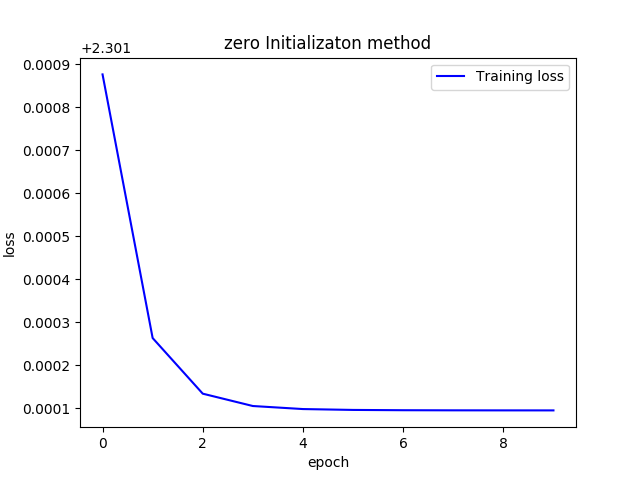
\includegraphics[width=1\textwidth]{zero_init.png}
\caption{\label{fig:init1}average loss against the training time (epoch) using zero initialization method.}
\end{figure}

\begin{figure}
\centering
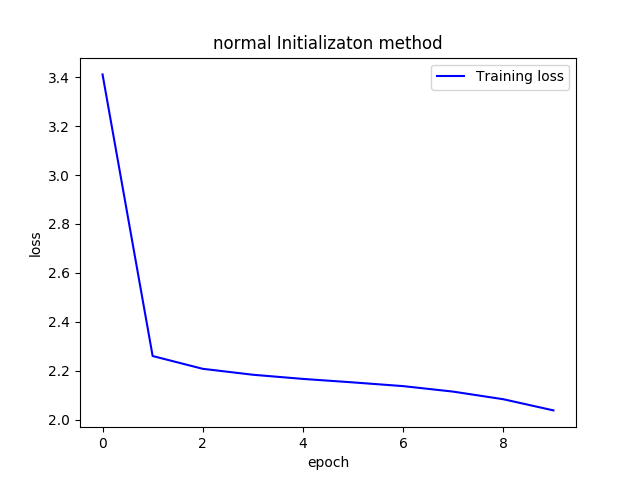
\includegraphics[width=1\textwidth]{normal_init.png}
\caption{\label{fig:init2}average loss against the training time (epoch) using normal initialization method.}
\end{figure}

\begin{figure}
\centering
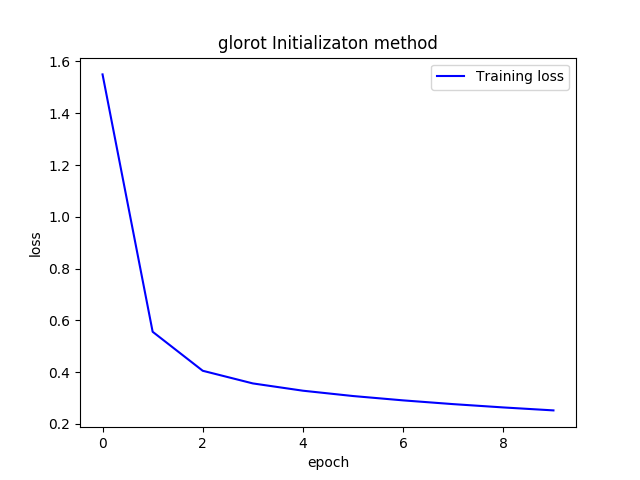
\includegraphics[width=1\textwidth]{glorot_init.png}
\caption{\label{fig:init3}average loss against the training time (epoch) using glorot initialization method.}
\end{figure}

\subsection{Hyperparameter Search}

\begin{enumerate}

\item
The combination of hyper-parameters that we found in which the average accuracy rate on the validation set reach 97.2\% accuracy:
A network with 2 hidden layers h1 = 64 hidden units and h2 = 32 hidden units with a total number of parameters of 52650. A Relu activation function, a learning rate of 0.01, a mini batch size of 64, a number of epochs of 50. (See Figure \ref{fig:lr1} plotting the training/validation accuracy over epochs).

\item 
We tried different hyper-parameters for learning rate, number of epochs {\color{red}{Number of epochs is not an hyperparameter, see slack channel tp1 01/29}}, network architecture and batch size. We consider the same model architecture.

\subsubsection{Learning rate}

We keep the same settings and we only change the learning rate.

\begin{itemize}

\item learning rate of 0.01: validation accuracy = 97.2\% (See Figure \ref{fig:lr1}).

\item learning rate of 0.1: validation accuracy = 97.6\% (See Figure \ref{fig:lr2}).

\item learning rate of 0.001: validation accuracy = 93\% (See Figure \ref{fig:lr3}).  
  
\end{itemize}

\begin{figure}
\centering
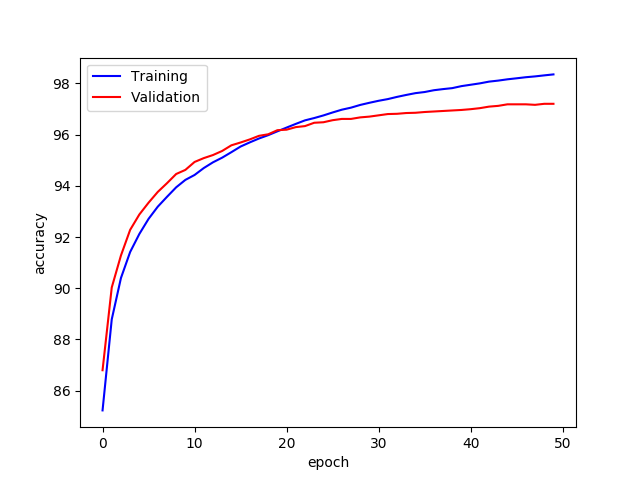
\includegraphics[width=1\textwidth]{acc_hyper.png}
\caption{\label{fig:hyper}Validation/training accuracy against the training time (epoch) using the chosen hyper-parameters.}
\end{figure}

\begin{figure}
\centering
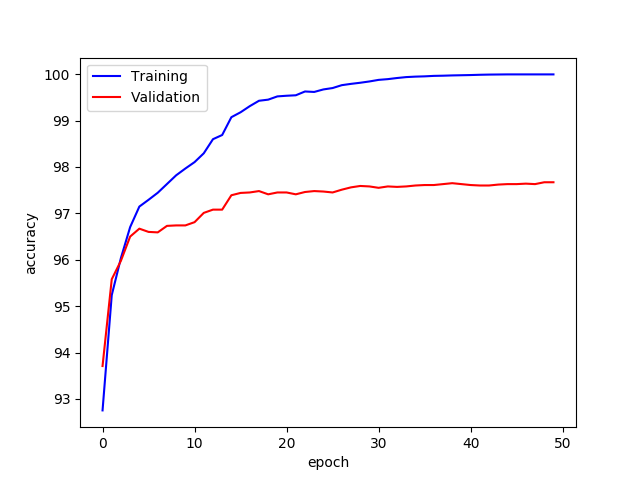
\includegraphics[width=1\textwidth]{lr2.png}
\caption{\label{fig:lr2}Validation accuracy against the training time (epoch) using a learning rate of 0.1.}
\end{figure}

\begin{figure}
\centering
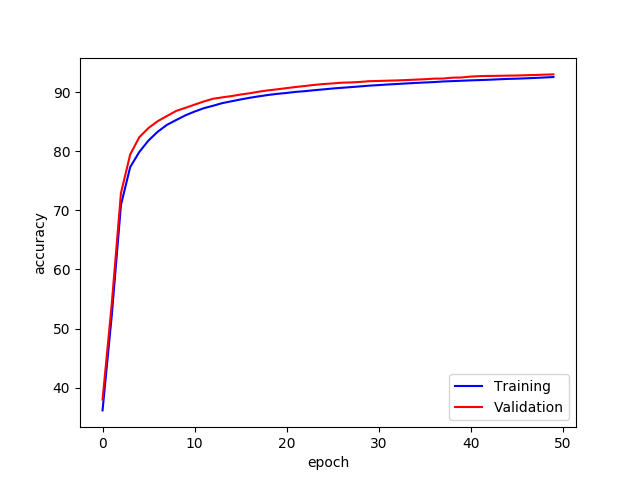
\includegraphics[width=1\textwidth]{lr3.png}
\caption{\label{fig:lr3}Validation accuracy against the training time (epoch) using a learning rate of 0.001.}
\end{figure}


\subsubsection{Number of epochs}
We keep the same settings and we only change the number of epochs.

\begin{itemize}

\item number of epochs of 50: validation accuracy = 97.2\% (See Figure \ref{fig:hyper}).

\item number of epochs of 5: validation accuracy = 92.8\% (See Figure \ref{fig:epoch2}).

\item number of epochs of 150: validation accuracy = 97.3\% (See Figure \ref{fig:epoch3}).  
  
\end{itemize}

\begin{figure}
\centering
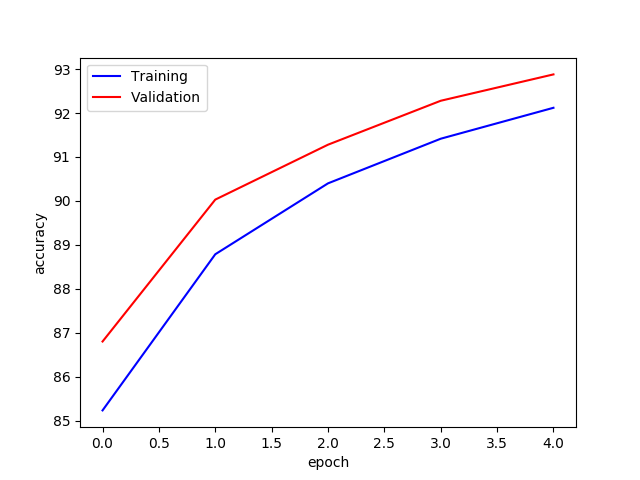
\includegraphics[width=1\textwidth]{epoch2.png}
\caption{\label{fig:epoch2}Validation/training accuracy against the training time (epoch) using a number of epochs of 5..}
\end{figure}

\begin{figure}
\centering
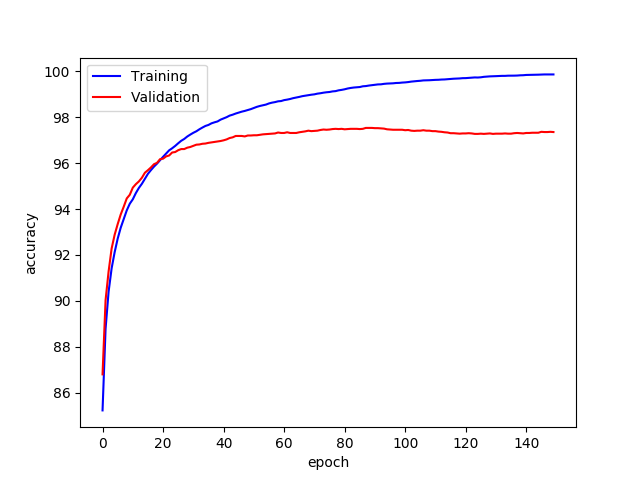
\includegraphics[width=1\textwidth]{epoch3.png}
\caption{\label{fig:epoch3}Validation/training accuracy against the training time (epoch) using a number of epochs of 150.}
\end{figure}

\subsubsection{Number of mini-batches}
We keep the same settings and we only change the number of mini-batches.

\begin{itemize}

\item number of mini-batches of 64: validation accuracy = 97.2\% (See Figure \ref{fig:hyper}).

\item number of mini-batches of 8: validation accuracy = 97.4\% (See Figure \ref{fig:batch2}).

\item number of mini-batches of 512: validation accuracy = 93.4\% (See Figure \ref{fig:batch3}).  
  
\end{itemize}

\begin{figure}
\centering
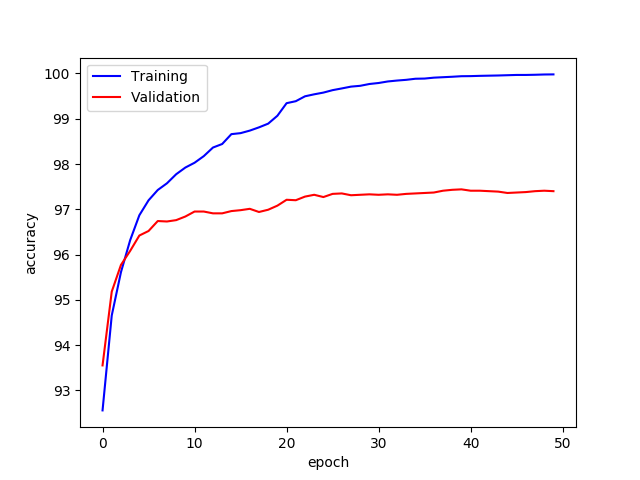
\includegraphics[width=1\textwidth]{batch2.png}
\caption{\label{fig:batch2}Validation/training accuracy against the training time (epoch) using a number of mini-batches of 8.}
\end{figure}

\begin{figure}
\centering
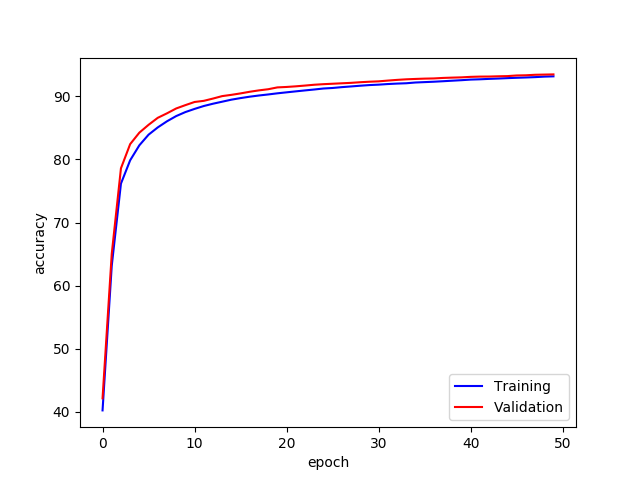
\includegraphics[width=1\textwidth]{batch3.png}
\caption{\label{fig:batch3}Validation/training accuracy against the training time (epoch) using a number of mini-batches of 512.}
\end{figure}

\subsubsection{Non-linearity activation function}
We keep the same settings and we only change the activation function.

\begin{itemize}

\item Relu activation function: validation accuracy = 97.2\% (See Figure \ref{fig:hyper}).

\item Sigmoid activation function: validation accuracy = 92.2\% (See Figure \ref{fig:sigmoid}).

\item tanh activation function: validation accuracy = 93.9\% (See Figure \ref{fig:tanh}).  
  
\end{itemize}

\begin{figure}
\centering
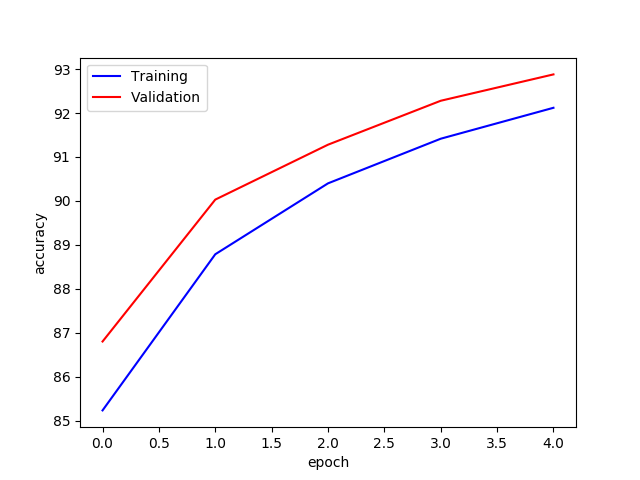
\includegraphics[width=1\textwidth]{epoch2.png}
\caption{\label{fig:sigmoid}Validation/training accuracy against the training time (epoch) using a sigmoid activation function.}
\end{figure}

\begin{figure}
\centering
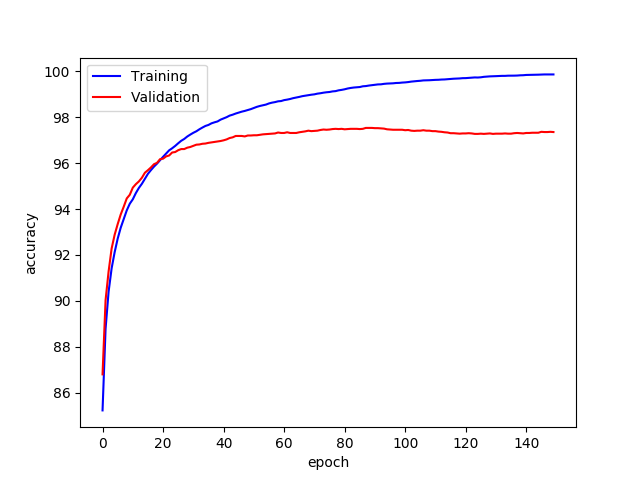
\includegraphics[width=1\textwidth]{epoch3.png}
\caption{\label{fig:tanh}Validation/training accuracy against the training time (epoch) using a tanh activation function.}
\end{figure}

\subsubsection{Network architecture (number of hidden units)}
We keep the same settings and we only change the hidden layers dimensions.

\begin{itemize}

\item Network with 2 hidden layers h1 = 64, h2 = 32: validation accuracy = 97.2\% (See Figure \ref{fig:hyper}).

\item Sigmoid activation function: validation accuracy = 92.2\% (See Figure \ref{fig:lr2}).

\item tanh activation function: validation accuracy = 93.9\% (See Figure \ref{fig:lr3}).  
  
\end{itemize}


\end{enumerate}

\section{Problem 2}
\label{sec:problem1}

\section{Problem 3 (Kaggle challenge)}
\label{sec:problem1}


\begin{thebibliography}
@online{,
  author = {Thayumanav Jayadevan},
  title = {Why don't we initialize the weights of a neural network to zero?},
  year = 2018,
  url = {https://www.quora.com/Why-dont-we-initialize-the-weights-of-a-neural-network-to-zero},
  urldate = {2019-02-05}
}
\end{thebibliography}
\end{document}